\documentclass[11pt,a4paper]{article}

\usepackage{main}
\usepackage{cours}

\usepackage{tikz}
\usetikzlibrary{positioning}

\renewcommand{\typedocument}{Cours}
\renewcommand{\classe}{6e}
\renewcommand{\titre}{Mouvement}

\begin{document}

\pagination

\creertitre{Mouvement et vitesse}

\partie{Le mouvement}

On appelle \important{mouvement} le déplacement d’un objet par rapport à un observateur.

On décrit toujours un mouvement par rapport à un objet ou une personne. On l’appelle le \important{référentiel}.

On appelle \important{trajectoire} le chemin suivi par l’objet au cours du temps.

\begin{itemize}
    \item Si la trajectoire est un \textbf{cercle}, alors le mouvement est \important{circulaire}.
    \item[] \exemple{La Terre autour du Soleil}
    \item Si la trajectoire est une \textbf{droite}, alors le mouvement est \important{rectiligne}.
    \item[] \exemple{Une voiture sur une ligne droite} 
\end{itemize}

\partie{La vitesse}

La \important{vitesse} moyenne d’un objet correspond à la distance parcourue par l’objet divisée par la durée du mouvement.

% \begin{center}
%     \LARGE\important{vitesse = distance / temps}
% \end{center}

\begin{center}
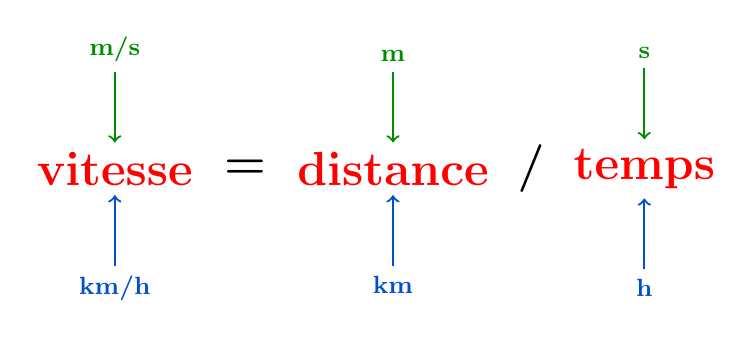
\begin{tikzpicture}[baseline=(current bounding box.center)]
  % Définition des couleurs
  \definecolor{vertfonce}{RGB}{0,140,0}
  \definecolor{bleufonce}{RGB}{0,80,200}

  % Nœuds de l'équation
  \node[font=\LARGE\bfseries\color{red}] (vitesse) {vitesse};
  \node[font=\LARGE\bfseries, right=0.15cm of vitesse] (egal) {=};
  \node[font=\LARGE\bfseries\color{red}, right=0.15cm of egal] (distance) {distance};
  \node[font=\LARGE\bfseries, right=0.12cm of distance] (div) {/};
  \node[font=\LARGE\bfseries\color{red}, right=0.12cm of div] (temps) {temps};

  % --- Annotations VERTES (m, s, m/s) au-dessus ---
  % Flèche verte vers "distance" → m
  \node[font=\small\bfseries, color=vertfonce, above=0.9cm of distance] (dm) {m};
  \draw[->, color=vertfonce, thick] (dm.south) -- (distance.north);

  % Flèche verte vers "temps" → s
  \node[font=\small\bfseries, color=vertfonce, above=0.9cm of temps] (ts) {s};
  \draw[->, color=vertfonce, thick] (ts.south) -- (temps.north);

  % Flèche verte vers "vitesse" → m/s
  \node[font=\small\bfseries, color=vertfonce, above=0.9cm of vitesse] (vms) {m/s};
  \draw[->, color=vertfonce, thick] (vms.south) -- (vitesse.north);

  % --- Annotations BLEUES (km, h, km/h) en dessous ---
  % Flèche bleue vers "distance" → km
  \node[font=\small\bfseries, color=bleufonce, below=0.9cm of distance] (dkm) {km};
  \draw[->, color=bleufonce, thick] (dkm.north) -- (distance.south);

  % Flèche bleue vers "temps" → h
  \node[font=\small\bfseries, color=bleufonce, below=0.9cm of temps] (th) {h};
  \draw[->, color=bleufonce, thick] (th.north) -- (temps.south);

  % Flèche bleue vers "vitesse" → km/h
  \node[font=\small\bfseries, color=bleufonce, below=0.9cm of vitesse] (vkmh) {km/h};
  \draw[->, color=bleufonce, thick] (vkmh.north) -- (vitesse.south);

\end{tikzpicture}
\end{center}

Le symbole de la vitesse est $v$.

L'unité de la vitesse peut-être le \textbf{mètre par seconde (m/s)} ou le \textbf{kilomètre par heure (km/h)}. Cela dépend des unités utilisées pour la distance et le temps.

On écrit plus simplement la formule de la vitesse : \important{$v = \frac{d}{t}$}, où d est la distance parcourue et t la durée du mouvement, exprimés dans les bonnes unités.

\begin{itemize}
    \item Si la vitesse est \textbf{constante}, le mouvement est \important{uniforme} (l’objet va toujours à la même vitesse).
    \item Si la vitesse \textbf{augmente}, le mouvement est \important{accéléré} (l’objet va de plus en plus vite).
    \item Si la vitesse \textbf{diminue}, le mouvement est \important{ralenti} (l’objet va de moins en moins vite).
\end{itemize}

\partie{A retenir}

Pour décrire le mouvement d’un objet, il faut préciser :

\begin{itemize}
    \item le référentiel choisi,
    \item la trajectoire de l’objet,
    \item sa vitesse.
\end{itemize}

\end{document}